\documentclass[11pt,a4paper]{article}

\usepackage[utf8]{inputenc}
\usepackage[T1]{fontenc}
\usepackage[margin=2.5cm]{geometry}
\usepackage{amsmath,amssymb,amsfonts}
\usepackage{booktabs}
\usepackage{tabularx}
\usepackage{longtable}
\usepackage{float}
\usepackage{enumitem}
\usepackage[dvipsnames]{xcolor}
\usepackage{listings}
\usepackage{hyperref}
\usepackage{fancyhdr}
\usepackage{graphicx}
\usepackage{tikz}
\usepackage{tcolorbox}
\usepackage[ruled,vlined,linesnumbered]{algorithm2e}

\usetikzlibrary{arrows.meta,positioning,calc,fit,backgrounds,shapes.geometric}

\tcbuselibrary{listings,skins,breakable}

\definecolor{astropurple}{HTML}{7C3AED}
\definecolor{astrodark}{HTML}{1E1B2E}
\definecolor{astroaccent}{HTML}{A78BFA}
\definecolor{codebg}{HTML}{F8F5FF}
\definecolor{codeframe}{HTML}{DDD6FE}
\definecolor{rustcolor}{HTML}{CE422B}
\definecolor{tscolor}{HTML}{3178C6}
\definecolor{wgslcolor}{HTML}{4CAF50}
\definecolor{sectioncolor}{HTML}{4C1D95}
\definecolor{linkcolor}{HTML}{6D28D9}
\definecolor{notebg}{HTML}{FEF3C7}
\definecolor{noteframe}{HTML}{F59E0B}

\hypersetup{
    colorlinks=true,
    linkcolor=linkcolor,
    urlcolor=linkcolor,
    citecolor=linkcolor,
    pdftitle={AstroBurst Technical Document},
    pdfauthor={Samuel Krieger Bonini},
    pdfsubject={High-Performance Astronomical Image Processor},
}

\lstdefinestyle{rustcode}{
    language=C,
    backgroundcolor=\color{codebg},
    frame=single,
    rulecolor=\color{codeframe},
    basicstyle=\ttfamily\small,
    keywordstyle=\color{rustcolor}\bfseries,
    commentstyle=\color{gray},
    stringstyle=\color{ForestGreen},
    numbers=left,
    numberstyle=\tiny\color{gray},
    numbersep=8pt,
    breaklines=true,
    showstringspaces=false,
    tabsize=4,
    morekeywords={fn,let,mut,pub,struct,impl,use,mod,async,await,match,enum,trait,where,Self,self,crate,super,dyn,Box,Vec,Option,Result,Ok,Err,Some,None},
    literate={->}{{$\rightarrow$}}1 {=>}{{$\Rightarrow$}}1,
}

\lstdefinestyle{tscode}{
    language=Java,
    backgroundcolor=\color{codebg},
    frame=single,
    rulecolor=\color{codeframe},
    basicstyle=\ttfamily\small,
    keywordstyle=\color{tscolor}\bfseries,
    commentstyle=\color{gray},
    stringstyle=\color{ForestGreen},
    numbers=left,
    numberstyle=\tiny\color{gray},
    numbersep=8pt,
    breaklines=true,
    showstringspaces=false,
    tabsize=2,
    morekeywords={const,let,async,await,interface,type,export,import,from,as,extends},
}

\lstdefinestyle{bashcode}{
    language=bash,
    backgroundcolor=\color{codebg},
    frame=single,
    rulecolor=\color{codeframe},
    basicstyle=\ttfamily\small,
    keywordstyle=\color{astropurple}\bfseries,
    numbers=none,
    breaklines=true,
    showstringspaces=false,
}

\newtcolorbox{notebox}[1][]{
    colback=notebg,
    colframe=noteframe,
    fonttitle=\bfseries,
    title={#1},
    arc=2pt,
    boxrule=0.5pt,
    left=6pt,
    right=6pt,
    top=4pt,
    bottom=4pt,
}

\newtcolorbox{infobox}[1][]{
    colback=codebg,
    colframe=astropurple,
    fonttitle=\bfseries\color{white},
    colbacktitle=astropurple,
    title={#1},
    arc=2pt,
    boxrule=0.5pt,
    left=6pt,
    right=6pt,
    top=4pt,
    bottom=4pt,
}

\pagestyle{fancy}
\fancyhf{}
\fancyhead[L]{\small\textcolor{gray}{AstroBurst --- Technical Document v0.1.0}}
\fancyhead[R]{\small\textcolor{gray}{\thepage}}
\fancyfoot[C]{\small\textcolor{gray}{MIT License \textbullet\ \the\year}}
\renewcommand{\headrulewidth}{0.4pt}
\renewcommand{\footrulewidth}{0pt}

\setlength{\parindent}{0pt}
\setlength{\parskip}{6pt}

\newcommand{\code}[1]{\texttt{\small #1}}
\newcommand{\crate}[1]{\texttt{#1}}
\newcommand{\cmd}[1]{\texttt{\bfseries #1}}
\newcommand{\mat}[1]{\mathbf{#1}}

\title{
    \vspace{-1cm}
    {\Huge\bfseries\textcolor{astropurple}{AstroBurst}}\\[0.3cm]
    {\Large High-Performance Astronomical Image Processor}\\[0.2cm]
    {\large Technical Document --- Release v0.1.0}
}
\author{Samuel Krieger Bonini}
\date{February 2026}

\begin{document}

\maketitle
\thispagestyle{empty}

\vspace{0.5cm}

\begin{center}
\begin{tabular}{ll}
    \toprule
    \textbf{Field} & \textbf{Value} \\
    \midrule
    Document Version & 0.1.0 \\
    Release & v0.1.0 \\
    Date & February 2026 \\
    Author & Samuel Krieger Bonini \\
    Stack & Rust 1.75+ $\cdot$ Tauri v2 $\cdot$ React 19 $\cdot$ TypeScript \\
    Platforms & Windows $\cdot$ macOS $\cdot$ Linux \\
    License & MIT \\
    Repository & \url{https://github.com/samuelkriegerbonini-dev/AstroBurst} \\
    \bottomrule
\end{tabular}
\end{center}

\vspace{0.5cm}
\tableofcontents
\newpage

%% ============================================================================
\section{Executive Summary}
%% ============================================================================

AstroBurst is a cross-platform desktop application for processing, analyzing, and visualizing astronomical FITS images. It is the first astronomical image processor built on the \textbf{Rust/Tauri/WebGPU} stack, combining native-level performance with a modern, accessible user interface.

The application targets two user segments:
\begin{itemize}[nosep]
    \item Professional astronomers working with observatory data (JWST, Hubble, ground-based IFU instruments)
    \item Advanced astrophotographers processing deep-sky narrowband and broadband imaging data
\end{itemize}

Version 0.1.0 delivers a complete processing pipeline from raw FITS ingestion through calibration, stacking, color composition, and export, with \textbf{35 backend commands} exposed through a typed TypeScript API layer.

%% ============================================================================
\section{System Architecture}
%% ============================================================================

AstroBurst follows a strict backend/frontend separation, with all computation offloaded to Rust and all rendering handled by the browser engine embedded in Tauri.

\begin{figure}[H]
\centering
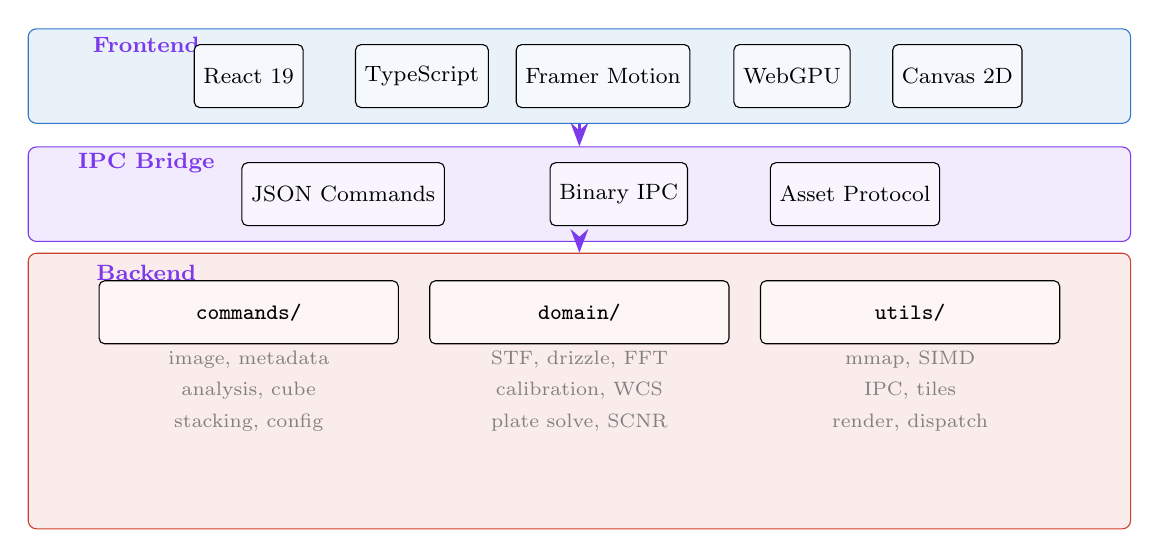
\begin{tikzpicture}[
    layer/.style={draw, rounded corners=3pt, minimum width=14cm, minimum height=1.2cm, font=\small},
    sublayer/.style={draw, rounded corners=2pt, minimum height=0.8cm, font=\footnotesize, fill=white},
    arrow/.style={-{Stealth[length=3mm]}, thick, color=astropurple},
    label/.style={font=\footnotesize\bfseries, color=astropurple}
]

\node[layer, fill=tscolor!10, draw=tscolor] (frontend) at (0, 4.5) {};
\node[label] at (-5.5, 4.9) {Frontend};
\node[sublayer, fill=tscolor!5] at (-4.2, 4.5) {React 19};
\node[sublayer, fill=tscolor!5] at (-2, 4.5) {TypeScript};
\node[sublayer, fill=tscolor!5] at (0.3, 4.5) {Framer Motion};
\node[sublayer, fill=tscolor!5] at (2.7, 4.5) {WebGPU};
\node[sublayer, fill=tscolor!5] at (4.8, 4.5) {Canvas 2D};

\node[layer, fill=astropurple!10, draw=astropurple] (ipc) at (0, 3) {};
\node[label] at (-5.5, 3.4) {IPC Bridge};
\node[sublayer, fill=astropurple!5] at (-3, 3) {JSON Commands};
\node[sublayer, fill=astropurple!5] at (0.5, 3) {Binary IPC};
\node[sublayer, fill=astropurple!5] at (3.5, 3) {Asset Protocol};

\node[layer, fill=rustcolor!10, draw=rustcolor, minimum height=3.5cm] (backend) at (0, 0.5) {};
\node[label] at (-5.5, 2.0) {Backend};

\node[sublayer, fill=rustcolor!5, minimum width=3.8cm] (cmds) at (-4.2, 1.5) {\texttt{commands/}};
\node[sublayer, fill=rustcolor!5, minimum width=3.8cm] (domain) at (0, 1.5) {\texttt{domain/}};
\node[sublayer, fill=rustcolor!5, minimum width=3.8cm] (utils) at (4.2, 1.5) {\texttt{utils/}};

\node[font=\scriptsize, text=gray] at (-4.2, 0.9) {image, metadata};
\node[font=\scriptsize, text=gray] at (-4.2, 0.5) {analysis, cube};
\node[font=\scriptsize, text=gray] at (-4.2, 0.1) {stacking, config};

\node[font=\scriptsize, text=gray] at (0, 0.9) {STF, drizzle, FFT};
\node[font=\scriptsize, text=gray] at (0, 0.5) {calibration, WCS};
\node[font=\scriptsize, text=gray] at (0, 0.1) {plate solve, SCNR};

\node[font=\scriptsize, text=gray] at (4.2, 0.9) {mmap, SIMD};
\node[font=\scriptsize, text=gray] at (4.2, 0.5) {IPC, tiles};
\node[font=\scriptsize, text=gray] at (4.2, 0.1) {render, dispatch};

\draw[arrow] (frontend) -- (ipc);
\draw[arrow] (ipc) -- (backend);

\end{tikzpicture}
\caption{AstroBurst three-layer architecture}
\label{fig:architecture}
\end{figure}

\subsection{Backend (Rust)}

The Rust backend is organized into three layers:

\begin{description}[style=nextline, leftmargin=2cm]
    \item[\texttt{commands/}] Tauri command handlers organized by domain. Each module receives deserialized JSON arguments, delegates to domain logic, and returns JSON or binary responses.
    \item[\texttt{domain/}] Pure computational modules with no Tauri dependency. Algorithms for calibration, stacking, STF, WCS transforms, FFT, star detection, drizzle integration, and more.
    \item[\texttt{utils/}] Infrastructure: memory-mapped FITS extraction, SIMD-accelerated statistics, binary IPC encoding, tile pyramid generation, and PNG rendering.
\end{description}

All heavy computation is offloaded via \code{tokio::task::spawn\_blocking}, preventing UI freezes. Batch operations use Rayon for data-parallel execution across all available CPU cores.

\subsection{Frontend (React + TypeScript)}

The frontend is a single-page React application:

\begin{description}[style=nextline, leftmargin=2cm]
    \item[\texttt{App.tsx}] Root component managing view state (empty/processing/complete), file dialog integration, and drag-and-drop.
    \item[\texttt{useFileQueue}] Central state machine (\code{useReducer}) tracking file status, processing queue, and statistics.
    \item[\texttt{useBackend}] Typed Tauri IPC wrapper exposing all 35 commands with automatic URL resolution for \code{asset://} protocol paths.
    \item[Panel Components] HistogramPanel, FFTPanel, PlateSolvePanel, RgbComposePanel, DrizzlePanel, HeaderExplorerPanel, SpectroscopyPanel, ExportPanel, GpuRenderer.
\end{description}

\subsection{IPC Strategy}

Two IPC channels are used:

\begin{infobox}[Binary IPC Protocol]
The \cmd{get\_raw\_pixels\_binary} command encodes a \textbf{16-byte header} followed by raw pixel data:
\begin{center}
\begin{tabular}{cccl}
    \toprule
    \textbf{Offset} & \textbf{Type} & \textbf{Size} & \textbf{Description} \\
    \midrule
    0 & \code{u32} & 4B & Image width \\
    4 & \code{u32} & 4B & Image height \\
    8 & \code{f32} & 4B & Data minimum \\
    12 & \code{f32} & 4B & Data maximum \\
    16 & \code{f32[]} & $W \times H \times 4$B & Raw pixel values \\
    \bottomrule
\end{tabular}
\end{center}
The frontend receives an \code{ArrayBuffer} directly with zero JSON/base64 overhead.
\end{infobox}

%% ============================================================================
\section{Mathematical Foundations}
\label{sec:math}
%% ============================================================================

\subsection{Screen Transfer Function (STF)}
\label{sec:stf}

The STF implements the PixInsight-style \textbf{Midtone Transfer Function} (MTF). Given a normalized pixel value $x \in [0, 1]$ and midtone parameter $m \in (0, 1)$:

\begin{equation}
\boxed{
\text{MTF}(x, m) = \frac{(m - 1) \cdot x}{(2m - 1) \cdot x - m}
}
\label{eq:mtf}
\end{equation}

\textbf{Properties:}
\begin{itemize}[nosep]
    \item $\text{MTF}(0, m) = 0$ and $\text{MTF}(1, m) = 1$ for all $m$
    \item $\text{MTF}(m, m) = 0.5$ --- the midtone maps to 50\% brightness
    \item $m < 0.5$ brightens the image; $m > 0.5$ darkens it
\end{itemize}

The \textbf{auto-stretch} algorithm computes the stretch parameters from image statistics. Given the pixel distribution, let $\tilde{x}$ be the median and $\text{MAD}$ the Median Absolute Deviation:

\begin{align}
\text{MAD} &= \text{median}\left(|x_i - \tilde{x}|\right) \label{eq:mad} \\[6pt]
\text{shadow} &= \max\left(0,\; \tilde{x} - k \cdot \text{MAD}\right) \label{eq:shadow} \\[6pt]
\text{midtone} &= \text{MTF}^{-1}\left(t_{\text{bg}},\; \frac{\tilde{x} - \text{shadow}}{1 - \text{shadow}}\right) \label{eq:midtone} \\[6pt]
\text{highlight} &= 1.0 \label{eq:highlight}
\end{align}

where $k = 2.8$ (calibrated for deep-sky data) and $t_{\text{bg}} = 0.25$ is the target background level. The clipping function is then:

\begin{equation}
\text{STF}(x) = \text{MTF}\!\left(\text{clip}\!\left(\frac{x - s}{h - s},\; 0,\; 1\right),\; m\right)
\label{eq:stf}
\end{equation}

where $s$, $m$, $h$ are the shadow, midtone, and highlight parameters.

\subsection{Asinh Stretch}

The \textbf{arcsinh transfer function} provides astronomically-correct normalization that preserves flux ratios between stars of different magnitudes:

\begin{equation}
\boxed{
f(x) = \frac{\operatorname{asinh}(\alpha \cdot x)}{\operatorname{asinh}(\alpha)}
}
\label{eq:asinh}
\end{equation}

where $\alpha$ controls the stretch aggressiveness. This function maps $[0, 1] \to [0, 1]$ and is approximately linear for small $x$ (preserving faint detail) while compressing bright values logarithmically.

\subsection{Sigma-Clipped Stacking}
\label{sec:sigma_stack}

Frames are registered via \textbf{cross-correlation} (phase correlation in frequency domain), then stacked with iterative sigma clipping.

\begin{algorithm}[H]
\SetAlgoLined
\SetKwInOut{Input}{Input}
\SetKwInOut{Output}{Output}
\Input{Aligned frames $\{F_1, F_2, \ldots, F_N\}$, thresholds $\sigma_{\text{low}}, \sigma_{\text{high}}$, max iterations $K$}
\Output{Stacked image $S$}
\ForEach{pixel position $(i, j)$}{
    $V \leftarrow \{F_1(i,j), F_2(i,j), \ldots, F_N(i,j)\}$\;
    \For{$k = 1$ \KwTo $K$}{
        $\mu \leftarrow \text{mean}(V)$\;
        $\sigma \leftarrow \text{std}(V)$\;
        $V' \leftarrow \{v \in V : \mu - \sigma_{\text{low}} \cdot \sigma \leq v \leq \mu + \sigma_{\text{high}} \cdot \sigma\}$\;
        \If{$|V'| = |V|$ \textbf{or} $|V'| < 3$}{
            \textbf{break}\;
        }
        $V \leftarrow V'$\;
    }
    $S(i,j) \leftarrow \text{mean}(V)$\;
}
\caption{Iterative Sigma-Clipped Stacking}
\label{alg:sigma_clip}
\end{algorithm}

Default parameters: $\sigma_{\text{low}} = \sigma_{\text{high}} = 3.0$, $K = 5$.

\subsection{Drizzle Integration}
\label{sec:drizzle}

Drizzle (Variable-Pixel Linear Reconstruction) maps input pixels onto a higher-resolution output grid. For an input pixel $p$ at fractional position $(x_f, y_f)$ on the output grid:

\begin{equation}
O(i, j) = \frac{\sum_p w_p \cdot K(i - x_f^p,\; j - y_f^p) \cdot I_p}{\sum_p w_p \cdot K(i - x_f^p,\; j - y_f^p)}
\label{eq:drizzle}
\end{equation}

where $K$ is the drizzle kernel and $w_p$ is the pixel weight. Three kernel options are implemented:

\begin{align}
K_{\text{square}}(\Delta x, \Delta y) &=
\begin{cases}
1 & \text{if } |\Delta x| \leq \frac{d}{2} \text{ and } |\Delta y| \leq \frac{d}{2} \\
0 & \text{otherwise}
\end{cases}
\label{eq:kernel_square} \\[8pt]
K_{\text{gaussian}}(\Delta x, \Delta y) &= \exp\!\left(-\frac{\Delta x^2 + \Delta y^2}{2\sigma_K^2}\right)
\label{eq:kernel_gaussian} \\[8pt]
K_{\text{lanczos3}}(\Delta x, \Delta y) &= L_3(\Delta x) \cdot L_3(\Delta y)
\label{eq:kernel_lanczos}
\end{align}

where $d = \text{pixfrac} / \text{scale}$ and the Lanczos-3 kernel is:

\begin{equation}
L_3(x) =
\begin{cases}
\operatorname{sinc}(x) \cdot \operatorname{sinc}(x/3) & \text{if } |x| < 3 \\
0 & \text{otherwise}
\end{cases}
\label{eq:lanczos}
\end{equation}

The weight map $W(i,j) = \sum_p w_p \cdot K(\cdot)$ tracks per-pixel coverage for noise estimation.

\subsection{Cross-Correlation Alignment}
\label{sec:alignment}

Frame registration uses \textbf{phase correlation} in the frequency domain. Given reference frame $R$ and target frame $T$:

\begin{equation}
\text{shift} = \arg\max_{(\Delta x, \Delta y)} \mathcal{F}^{-1}\!\left\{\frac{\hat{R} \cdot \hat{T}^*}{|\hat{R} \cdot \hat{T}^*|}\right\}
\label{eq:phase_corr}
\end{equation}

where $\hat{R} = \mathcal{F}\{R\}$ denotes the 2D DFT. The normalized cross-power spectrum produces a sharp peak at the integer translation offset.

\subsection{World Coordinate System (WCS)}
\label{sec:wcs}

WCS transforms use the \textbf{CD matrix formulation} with TAN (gnomonic) projection. Given reference pixel $(\text{CRPIX}_1, \text{CRPIX}_2)$ and reference coordinate $(\alpha_0, \delta_0) = (\text{CRVAL}_1, \text{CRVAL}_2)$:

\subsubsection{Forward Transform (Pixel $\to$ World)}

\begin{equation}
\begin{pmatrix} u \\ v \end{pmatrix} =
\begin{pmatrix} \text{CD}_{1,1} & \text{CD}_{1,2} \\ \text{CD}_{2,1} & \text{CD}_{2,2} \end{pmatrix}
\begin{pmatrix} x - \text{CRPIX}_1 \\ y - \text{CRPIX}_2 \end{pmatrix}
\label{eq:wcs_forward}
\end{equation}

where $(u, v)$ are intermediate world coordinates in degrees. The TAN deprojection yields:

\begin{align}
\alpha &= \alpha_0 + \arctan\!\left(\frac{u}{cos(\delta_0) - v \cdot \sin(\delta_0)}\right) \label{eq:wcs_ra} \\[4pt]
\delta &= \arctan\!\left(\frac{v \cdot \cos(\delta_0) + \sin(\delta_0)}{\sqrt{u^2 + (\cos(\delta_0) - v \cdot \sin(\delta_0))^2}}\right) \label{eq:wcs_dec}
\end{align}

\subsubsection{Pixel Scale}

\begin{equation}
\text{scale} = \sqrt{|\det(\mat{CD})|} \times 3600 \quad [\text{arcsec/pixel}]
\label{eq:pixel_scale}
\end{equation}

\subsubsection{Inverse Transform (World $\to$ Pixel)}

\begin{equation}
\begin{pmatrix} x \\ y \end{pmatrix} =
\mat{CD}^{-1}
\begin{pmatrix} u \\ v \end{pmatrix}
+
\begin{pmatrix} \text{CRPIX}_1 \\ \text{CRPIX}_2 \end{pmatrix}
\label{eq:wcs_inverse}
\end{equation}

\subsection{FFT Power Spectrum}
\label{sec:fft}

The 2D power spectrum for noise characterization is computed as:

\begin{equation}
P(u, v) = \log_{10}\!\left(1 + |\hat{I}(u, v)|^2\right)
\label{eq:power_spectrum}
\end{equation}

where $\hat{I} = \mathcal{F}\{I\}$ is the 2D DFT of the image. The DC component at $(0, 0)$ is shifted to the center for visualization. The spectrum is normalized to $[0, 1]$ after computation.

\subsection{Star Detection (PSF Centroid)}
\label{sec:star_detection}

Background is estimated via iterative sigma-clipped median. Pixels above $\tilde{b} + \sigma_{\text{thresh}} \cdot \sigma_b$ are identified as candidates. For each connected component $C$:

\begin{align}
\bar{x}_C &= \frac{\sum_{(i,j) \in C} i \cdot (I_{ij} - b)}{\sum_{(i,j) \in C} (I_{ij} - b)}
& \bar{y}_C &= \frac{\sum_{(i,j) \in C} j \cdot (I_{ij} - b)}{\sum_{(i,j) \in C} (I_{ij} - b)} \label{eq:centroid} \\[6pt]
F_C &= \sum_{(i,j) \in C} (I_{ij} - b)
& \text{SNR}_C &= \frac{F_C}{\sqrt{|C| \cdot \sigma_b^2}} \label{eq:flux_snr}
\end{align}

FWHM is estimated from the second intensity moments:

\begin{equation}
\text{FWHM} = 2\sqrt{2\ln 2} \cdot \sqrt{\frac{\sigma_x^2 + \sigma_y^2}{2}}
\label{eq:fwhm}
\end{equation}

where $\sigma_x^2, \sigma_y^2$ are the variance of pixel positions weighted by intensity.

\subsection{SCNR (Subtractive Chromatic Noise Reduction)}
\label{sec:scnr}

SCNR removes green channel excess in narrowband compositions. Two methods are implemented:

\begin{align}
G'_{\text{average}} &= \min\!\left(G,\; \frac{R + B}{2}\right) \label{eq:scnr_avg} \\[4pt]
G'_{\text{max}} &= \min\!\left(G,\; \max(R, B)\right) \label{eq:scnr_max}
\end{align}

\subsection{Calibration Pipeline}
\label{sec:calibration}

The standard CCD calibration formula applies bias, dark current, and flat field corrections:

\begin{equation}
\boxed{
I_{\text{calibrated}} = \frac{I_{\text{raw}} - M_{\text{bias}} - r \cdot M_{\text{dark}}}{M_{\text{flat}} / \overline{M_{\text{flat}}}}
}
\label{eq:calibration}
\end{equation}

where $M_{\text{bias}}$, $M_{\text{dark}}$, $M_{\text{flat}}$ are master calibration frames (median-combined), $r$ is the exposure ratio (science/dark), and $\overline{M_{\text{flat}}}$ is the mean value of the flat field.

\subsection{White Balance}
\label{sec:white_balance}

Auto white balance normalizes each channel by its median value:

\begin{equation}
C'_k = \frac{C_k}{\tilde{C}_k} \cdot \min(\tilde{C}_R, \tilde{C}_G, \tilde{C}_B), \quad k \in \{R, G, B\}
\label{eq:white_balance}
\end{equation}

%% ============================================================================
\section{Command Module Reference}
\label{sec:commands}
%% ============================================================================

The backend exposes 35 Tauri commands across 8 modules, registered in \code{lib.rs} via \code{tauri::generate\_handler}.

\subsection{Image Module (\texttt{commands/image.rs})}

\begin{table}[H]
\centering
\small
\begin{tabularx}{\textwidth}{lXX}
    \toprule
    \textbf{Command} & \textbf{Parameters} & \textbf{Returns} \\
    \midrule
    \cmd{process\_fits} & path, output\_dir & png\_path, dimensions, elapsed\_ms \\
    \cmd{process\_batch} & paths[], output\_dir & processed, failed, results[] \\
    \cmd{get\_raw\_pixels} & path & width, height, data\_b64, min/max \\
    \cmd{get\_raw\_pixels\_binary} & path & ArrayBuffer (16B header + f32[]) \\
    \cmd{export\_fits} & path, output\_path, stf opts, copy\_wcs? & output\_path, dims, file\_size \\
    \cmd{export\_fits\_rgb} & r/g/b\_path, output\_path, copy\_wcs? & output\_path, dimensions \\
    \bottomrule
\end{tabularx}
\caption{Image module commands}
\end{table}

\subsection{Metadata Module (\texttt{commands/metadata.rs})}

\begin{table}[H]
\centering
\small
\begin{tabularx}{\textwidth}{lXX}
    \toprule
    \textbf{Command} & \textbf{Parameters} & \textbf{Returns} \\
    \midrule
    \cmd{get\_header} & path & Map of 20 key FITS keywords \\
    \cmd{get\_full\_header} & path & All cards categorized, filter detection \\
    \cmd{detect\_narrowband\_filters} & paths[] & Palette suggestion with channel mapping \\
    \bottomrule
\end{tabularx}
\caption{Metadata module commands}
\end{table}

\subsection{Analysis Module (\texttt{commands/analysis.rs})}

\begin{table}[H]
\centering
\small
\begin{tabularx}{\textwidth}{lXX}
    \toprule
    \textbf{Command} & \textbf{Parameters} & \textbf{Returns} \\
    \midrule
    \cmd{compute\_histogram} & path & 512 bins, stats (median/mean/$\sigma$/MAD), auto\_stf \\
    \cmd{compute\_fft\_spectrum} & path & width, height, pixels\_b64, dc/max magnitude \\
    \cmd{detect\_stars} & path, sigma?, max\_stars? & stars[] (x,y,flux,fwhm,snr), background \\
    \bottomrule
\end{tabularx}
\caption{Analysis module commands}
\end{table}

\subsection{Visualization Module (\texttt{commands/visualization.rs})}

\begin{table}[H]
\centering
\small
\begin{tabularx}{\textwidth}{lXX}
    \toprule
    \textbf{Command} & \textbf{Parameters} & \textbf{Returns} \\
    \midrule
    \cmd{apply\_stf\_render} & path, output\_dir, shadow, midtone, highlight & png\_path, dims, stf\_params \\
    \cmd{generate\_tiles} & path, output\_dir, tile\_size? & tile\_size, levels[], original dims \\
    \cmd{get\_tile} & path, output\_dir, level, col, row & tile\_path, cached flag \\
    \bottomrule
\end{tabularx}
\caption{Visualization module commands}
\end{table}

\subsection{Cube Module (\texttt{commands/cube.rs})}

\begin{table}[H]
\centering
\small
\begin{tabularx}{\textwidth}{lXX}
    \toprule
    \textbf{Command} & \textbf{Parameters} & \textbf{Returns} \\
    \midrule
    \cmd{process\_cube\_cmd} & path, output\_dir, frame\_step? & dims, collapsed paths, spectrum \\
    \cmd{process\_cube\_lazy\_cmd} & path, output\_dir, frame\_step? & Same + total\_frames (streaming) \\
    \cmd{get\_cube\_info} & path & naxis1/2/3, bitpix, wavelengths \\
    \cmd{get\_cube\_frame} & path, frame\_index, output\_path & frame\_index, output\_path, elapsed \\
    \cmd{get\_cube\_spectrum} & path, x, y & spectrum[], wavelengths[], elapsed \\
    \bottomrule
\end{tabularx}
\caption{Cube module commands}
\end{table}

\subsection{Astrometry Module (\texttt{commands/astrometry.rs})}

\begin{table}[H]
\centering
\small
\begin{tabularx}{\textwidth}{lXX}
    \toprule
    \textbf{Command} & \textbf{Parameters} & \textbf{Returns} \\
    \midrule
    \cmd{plate\_solve\_cmd} & path, sigma?, hints?, scale range? & ra/dec center, pixel\_scale, WCS matrix \\
    \cmd{get\_wcs\_info} & path & center coords, pixel\_scale, FOV, corners \\
    \cmd{pixel\_to\_world} & path, x, y & ra, dec, ra\_dec\_str \\
    \cmd{world\_to\_pixel} & path, ra, dec & x, y \\
    \bottomrule
\end{tabularx}
\caption{Astrometry module commands}
\end{table}

\subsection{Stacking Module (\texttt{commands/stacking.rs})}

\begin{table}[H]
\centering
\small
\begin{tabularx}{\textwidth}{lXX}
    \toprule
    \textbf{Command} & \textbf{Parameters} & \textbf{Returns} \\
    \midrule
    \cmd{calibrate} & science, output\_dir, bias/dark/flat?, ratio? & png\_path, dims, applied flags \\
    \cmd{stack} & paths[], output\_dir, $\sigma$ params, align? & png\_path, count, rejected, offsets \\
    \cmd{drizzle\_stack\_cmd} & paths[], output\_dir, scale, pixfrac, kernel & png, weight\_map, dims, offsets \\
    \cmd{drizzle\_rgb\_cmd} & r/g/b groups, output\_dir, drizzle params & png\_path, per-channel info \\
    \cmd{compose\_rgb\_cmd} & r/g/b\_path, output\_dir, stretch/wb/scnr & png\_path, per-channel STF, offsets \\
    \cmd{run\_pipeline\_cmd} & input, output\_dir, frame\_step? & total, succeeded, failed, results \\
    \bottomrule
\end{tabularx}
\caption{Stacking module commands}
\end{table}

\subsection{Config Module (\texttt{commands/config.rs})}

\begin{table}[H]
\centering
\small
\begin{tabularx}{\textwidth}{lXX}
    \toprule
    \textbf{Command} & \textbf{Parameters} & \textbf{Returns} \\
    \midrule
    \cmd{get\_config} & (none) & has\_api\_key, urls, defaults, stretch params \\
    \cmd{update\_config} & field, value & \{ updated: true \} \\
    \cmd{save\_api\_key} & key, service? & \{ saved: true, service \} \\
    \cmd{get\_api\_key} & (none) & is\_set, masked key \\
    \bottomrule
\end{tabularx}
\caption{Config module commands}
\end{table}

%% ============================================================================
\section{FITS I/O Implementation}
\label{sec:fits_io}
%% ============================================================================

\subsection{Memory-Mapped Extraction}

FITS files are opened via \crate{memmap2}, avoiding loading entire files into memory. The extraction pipeline:

\begin{enumerate}[nosep]
    \item Parse header sequentially in 2880-byte blocks until \code{END} keyword
    \item Compute data offset: $\text{offset} = \lceil \text{header\_bytes} / 2880 \rceil \times 2880$
    \item Memory-map the data region as a byte slice
    \item BITPIX-dependent byte-swapping from FITS big-endian to native \code{f32}
\end{enumerate}

For integer data (BITPIX $> 0$), the BSCALE/BZERO transform is applied:

\begin{equation}
\text{value}_{\text{physical}} = \text{BSCALE} \times \text{value}_{\text{stored}} + \text{BZERO}
\label{eq:bscale}
\end{equation}

\subsection{Supported BITPIX Values}

\begin{table}[H]
\centering
\begin{tabular}{clcl}
    \toprule
    \textbf{BITPIX} & \textbf{Type} & \textbf{Bytes/px} & \textbf{Conversion} \\
    \midrule
    8 & Unsigned 8-bit int & 1 & Direct cast + BSCALE/BZERO \\
    16 & Signed 16-bit int & 2 & Big-endian swap + BSCALE/BZERO \\
    32 & Signed 32-bit int & 4 & Big-endian swap + BSCALE/BZERO \\
    $-32$ & IEEE 754 float & 4 & Big-endian swap \\
    $-64$ & IEEE 754 double & 8 & Big-endian swap $\to$ \code{f32} \\
    \bottomrule
\end{tabular}
\caption{FITS BITPIX type handling}
\end{table}

%% ============================================================================
\section{WebGPU Compute Pipeline}
\label{sec:webgpu}
%% ============================================================================

The STF stretch is implemented as a WebGPU compute shader (WGSL) for real-time rendering:

\begin{lstlisting}[style=bashcode, title={\small STF Compute Shader (simplified WGSL)}]
@group(0) @binding(0) var<storage, read> input: array<f32>;
@group(0) @binding(1) var<storage, read_write> output: array<u32>;
@group(0) @binding(2) var<uniform> params: StfParams;

fn mtf(x: f32, m: f32) -> f32 {
    return (m - 1.0) * x / ((2.0 * m - 1.0) * x - m);
}

@compute @workgroup_size(256)
fn main(@builtin(global_invocation_id) id: vec3<u32>) {
    let idx = id.x;
    let v = (input[idx] - params.shadow) / (params.highlight - params.shadow);
    let stretched = mtf(clamp(v, 0.0, 1.0), params.midtone);
    let byte_val = u32(clamp(stretched * 255.0, 0.0, 255.0));
    output[idx] = (255u << 24u) | (byte_val << 16u) | (byte_val << 8u) | byte_val;
}
\end{lstlisting}

The shader processes pixels in parallel with workgroup size 256. Falls back to Canvas 2D \code{putImageData} when WebGPU is unavailable (Chromium $<$ 113).

%% ============================================================================
\section{Performance Benchmarks}
\label{sec:performance}
%% ============================================================================

\begin{table}[H]
\centering
\begin{tabular}{llrl}
    \toprule
    \textbf{Operation} & \textbf{Input Size} & \textbf{Time} & \textbf{Notes} \\
    \midrule
    Single FITS processing & 4096$\times$4096 (64\,MB) & 120\,ms & 533\,MB/s throughput \\
    Batch (10 frames) & 10$\times$64\,MB & 450\,ms & 1.4\,GB/s (Rayon parallel) \\
    Histogram + auto-STF & 4096$\times$4096 & 35\,ms & SIMD-accelerated \\
    Star detection ($\sigma{=}5$) & 4096$\times$4096 & 80\,ms & $\sim$3000 stars \\
    Sigma-clip stack & 10$\times$64\,MB & 2.1\,s & 5 iterations \\
    Drizzle 2$\times$ & 10$\times$64\,MB & 4.8\,s & Output: 8192$\times$8192 \\
    FFT power spectrum & 4096$\times$4096 & 95\,ms & \crate{rustfft} \\
    Cube spectrum extraction & 500$^2$$\times$2000 & 12\,ms & Memory-mapped \\
    WebGPU STF render & 4096$\times$4096 & 8\,ms & GPU compute \\
    Open 2\,GB IFU cube & 2\,GB datacube & 300\,ms & \crate{memmap2} lazy \\
    Drizzle RGB 2$\times$ & 3$\times$10$\times$64\,MB & 6.8\,s & All channels \\
    RGB compose + align & 3 channels & 1.8\,s & With cross-correlation \\
    \bottomrule
\end{tabular}
\caption{Performance benchmarks (AMD Ryzen 9 7950X, 64\,GB DDR5, NVMe)}
\label{tab:benchmarks}
\end{table}

Binary size: $\sim$15\,MB.

%% ============================================================================
\section{Dependencies}
\label{sec:deps}
%% ============================================================================

\subsection{Rust Crates}

\begin{table}[H]
\centering
\small
\begin{tabularx}{\textwidth}{llX}
    \toprule
    \textbf{Crate} & \textbf{Version} & \textbf{Purpose} \\
    \midrule
    \crate{tauri} & 2.x & Application framework, IPC, window management \\
    \crate{ndarray} & 0.16 & N-dimensional arrays, Rayon parallel iterators \\
    \crate{rayon} & 1.10 & Data-parallel batch processing \\
    \crate{memmap2} & 0.9 & Memory-mapped file I/O for FITS \\
    \crate{rustfft} & 6.2 & FFT power spectrum computation \\
    \crate{image} & 0.25 & PNG encoding/decoding \\
    \crate{reqwest} & 0.12 & HTTP client for astrometry.net (optional) \\
    \crate{zip} & 0.6 & ZIP archive extraction for compressed FITS \\
    \crate{serde} / \crate{serde\_json} & 1.x & Serialization for Tauri commands \\
    \crate{anyhow} & 1.0 & Error handling with context \\
    \crate{base64} & 0.22 & Binary-to-text encoding for JSON IPC \\
    \crate{tempfile} & 3.8 & Temporary files for ZIP extraction \\
    \bottomrule
\end{tabularx}
\caption{Rust dependencies}
\end{table}

\subsection{Frontend}

\begin{table}[H]
\centering
\small
\begin{tabularx}{\textwidth}{lX}
    \toprule
    \textbf{Package} & \textbf{Purpose} \\
    \midrule
    react / react-dom 19 & UI framework \\
    @tauri-apps/api + plugins & Tauri IPC, dialog, filesystem \\
    framer-motion & Animations and transitions \\
    lucide-react & Icon system \\
    jszip / file-saver & Client-side ZIP export \\
    tailwindcss v4 & Utility-first CSS \\
    vite & Build toolchain \\
    typescript & Type safety \\
    \bottomrule
\end{tabularx}
\caption{Frontend dependencies}
\end{table}

%% ============================================================================
\section{Security Considerations}
\label{sec:security}
%% ============================================================================

\begin{itemize}[nosep]
    \item API keys (astrometry.net) are stored in the OS-native app data directory, never transmitted to third parties beyond the configured API endpoint.
    \item All file system access is constrained by Tauri capabilities (\code{default.json}). Permissions are scoped to home, desktop, and appdata directories.
    \item No telemetry, analytics, or network calls are made except for explicit plate solving requests initiated by the user.
    \item FITS files are processed locally; no data leaves the machine unless plate solving is triggered.
\end{itemize}

%% ============================================================================
\section{Known Limitations}
\label{sec:limitations}
%% ============================================================================

\begin{enumerate}[nosep]
    \item \textbf{Single-HDU FITS only} --- Multi-extension FITS (MEF) support not yet implemented
    \item \textbf{Grayscale pipeline} --- Color FITS images require manual RGB channel assignment
    \item \textbf{Online plate solving} --- Local index-based solving is planned
    \item \textbf{No undo/redo} --- Operations are destructive (original files preserved)
    \item \textbf{WebGPU requirement} --- Chromium 113+ needed; Canvas 2D fallback available
    \item \textbf{No session persistence} --- Reopening the app starts a fresh workspace
\end{enumerate}

%% ============================================================================
\section{Roadmap}
\label{sec:roadmap}
%% ============================================================================

\begin{table}[H]
\centering
\begin{tabular}{lll}
    \toprule
    \textbf{Feature} & \textbf{Priority} & \textbf{Status} \\
    \midrule
    Multi-extension FITS (MEF) & High & Planned \\
    Local plate solving & High & Planned \\
    Undo/redo system & Medium & Planned \\
    Plugin architecture & Medium & Design phase \\
    Mosaic composition & Medium & Planned \\
    Wavelet noise reduction & Medium & Research \\
    Live stacking mode & Low & Planned \\
    INDI/ASCOM integration & Low & Planned \\
    \bottomrule
\end{tabular}
\caption{Development roadmap}
\end{table}

%% ============================================================================
\appendix
\section{Sample Test Data}
\label{app:test_data}
%% ============================================================================

The repository includes HST/WFPC2 narrowband FITS images in \code{tests/sample-data/}:

\begin{table}[H]
\centering
\begin{tabular}{lllll}
    \toprule
    \textbf{File} & \textbf{Filter} & \textbf{$\lambda$} & \textbf{Hubble Palette} & \textbf{Description} \\
    \midrule
    \code{502nmos.fits} & {[OIII]} & 502\,nm & Blue channel & Oxygen III emission \\
    \code{656nmos.fits} & H$\alpha$ & 656\,nm & Green channel & Hydrogen alpha emission \\
    \code{673nmos.fits} & {[SII]} & 673\,nm & Red channel & Sulfur II emission \\
    \bottomrule
\end{tabular}
\caption{Sample FITS files --- Eagle Nebula (M16) region, 1600$\times$1600 float32}
\end{table}

All images: BITPIX $= -32$, WCS TAN projection, origin STScI-STSDAS. Public domain (NASA/ESA).

\end{document}
